\section{Analysis of Performance}
\label{sec:analysis}

In this section, we assess the performance of our implementation through systematic benchmarking, controlled experimental evaluation, and quantitative analysis. We provide a comprehensive characterization of the computational cost of each model component, supported by a rigorous theoretical examination of the corresponding performance metrics. The objective of this study is to delineate the strengths and performance-limiting factors of the implementation, thereby yielding insights to inform and guide subsequent optimization efforts.
\begin{figure*}[!ht]
    \centering
    \begin{subfigure}
        {0.58\textwidth}
        \centering
        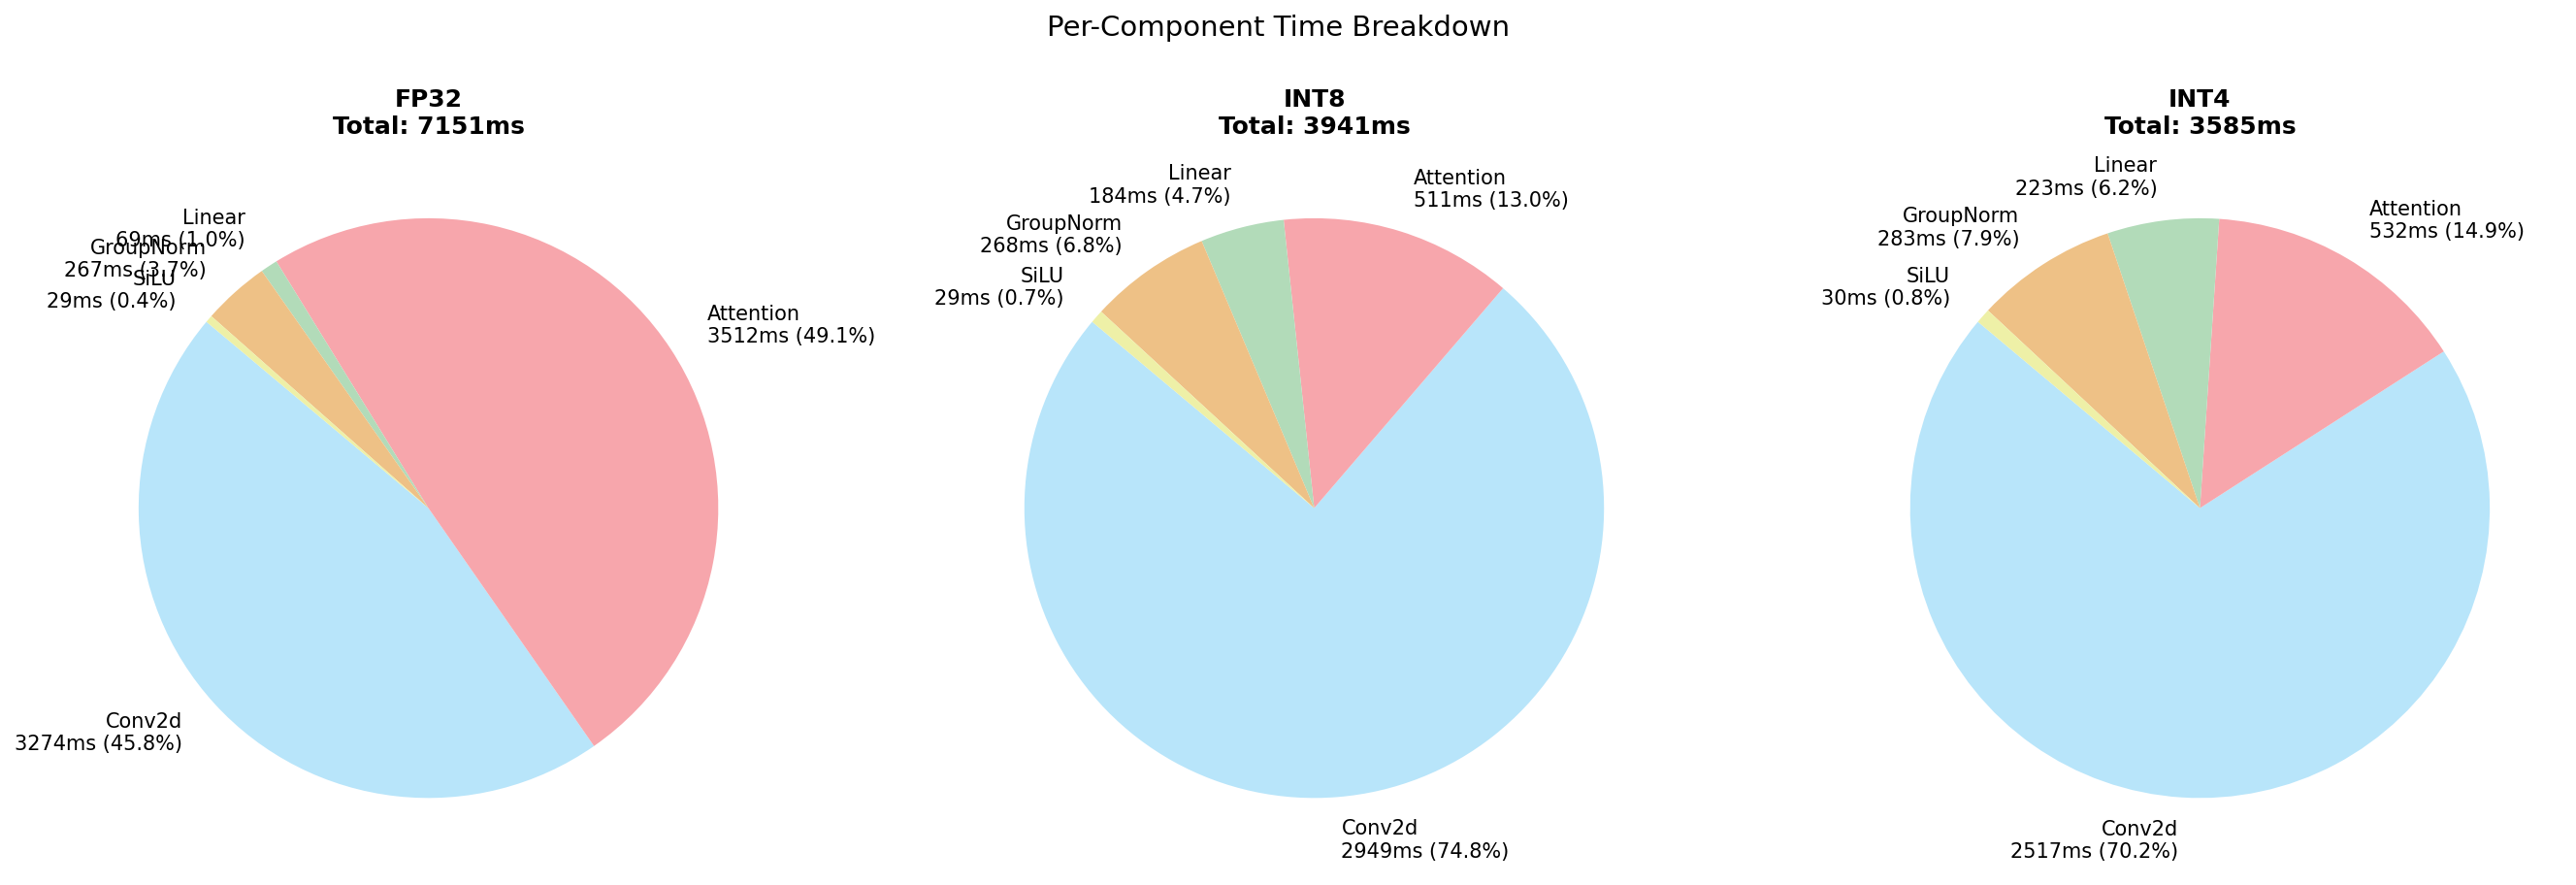
\includegraphics[width=\textwidth]{figures/plot_02_component_breakdown.png}
        \caption{Computational Cost Breakdown}
        \label{fig:plot_02}
    \end{subfigure}
    \hfill
    \begin{subfigure}
        {0.38\textwidth}
        \centering
        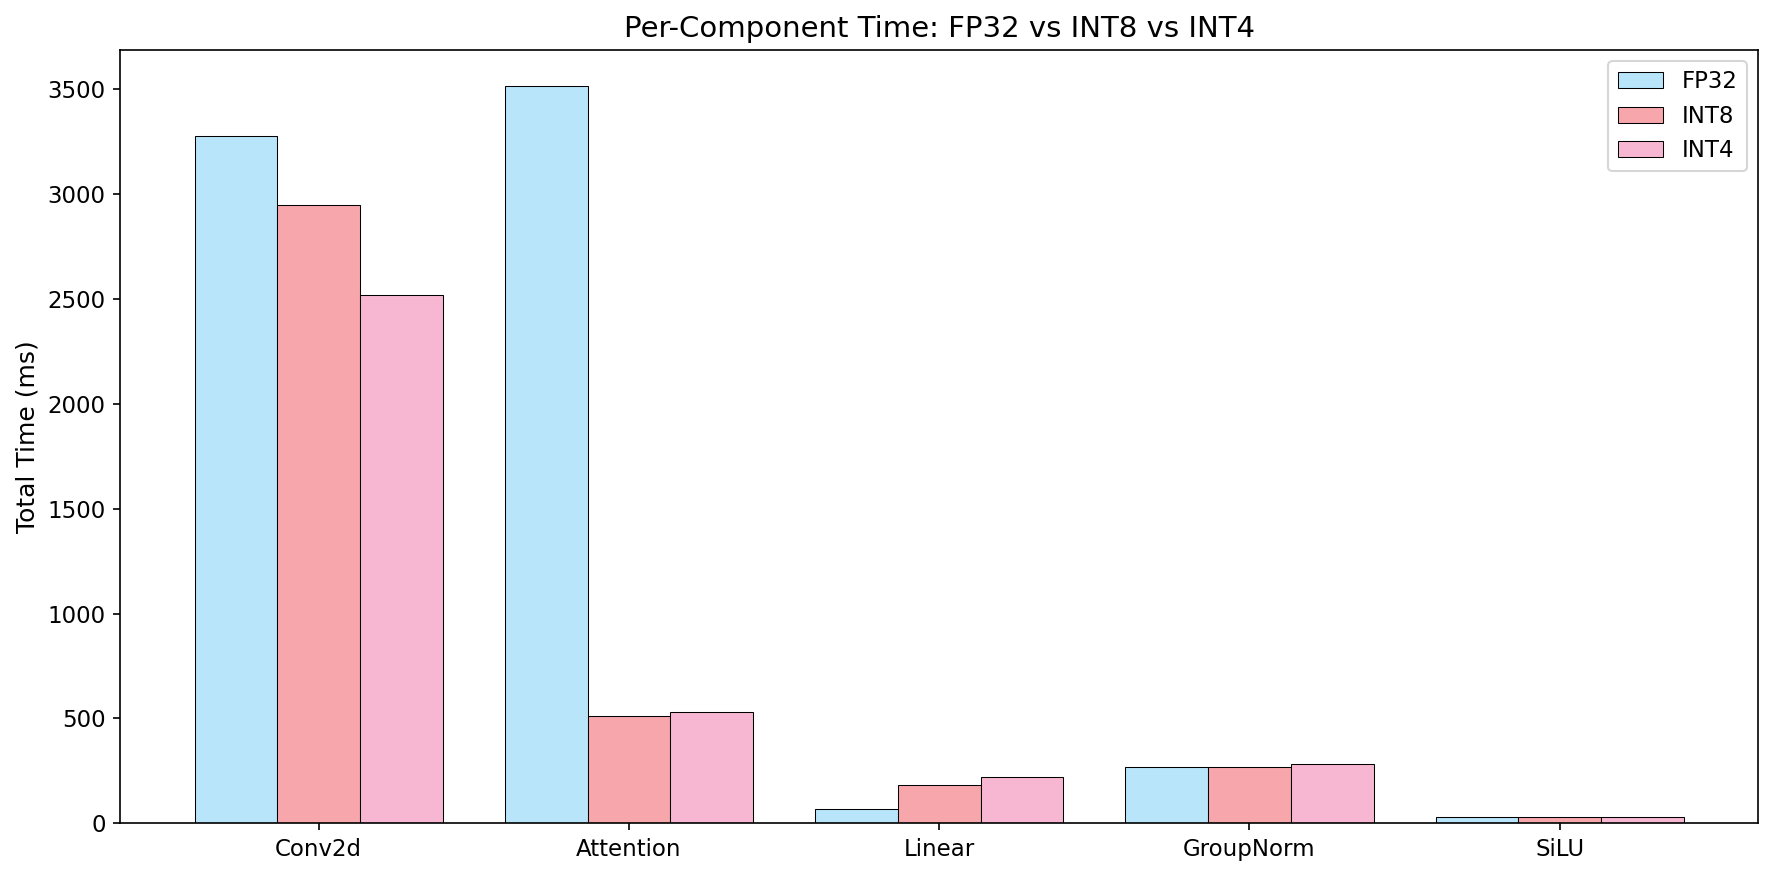
\includegraphics[width=\textwidth]{figures/plot_02b_component_bars.png}
        \caption{Computational Cost Breakdown (Bar Chart)}
        \label{fig:plot_02b}
    \end{subfigure}
    \caption{Computational Cost Breakdown}
    \label{fig:compu_cost_breakdown}
\end{figure*}

\subsection{Computational Cost Breakdown}

To understand where time is spent, we break down component-level cumulative cost in Figure~\ref{fig:compu_cost_breakdown} and Table~\ref{tab:component_breakdown}.

Based on the detailed computational breakdown, we observe that convolutional and attention layers constitute the primary contributors to the overall computational cost. This suggests that the MoDiff optimization, which reduces the time spent on convolutional operations, can substantially decrease the required computational resources. Nevertheless, residual non-quantized layers still contribute non-negligibly to the total computation, which explains the optimization's inability to attain the theoretically optimal throughput of fully low-bit convolutional implementations.

\begin{figure*}[!t]
    \centering
    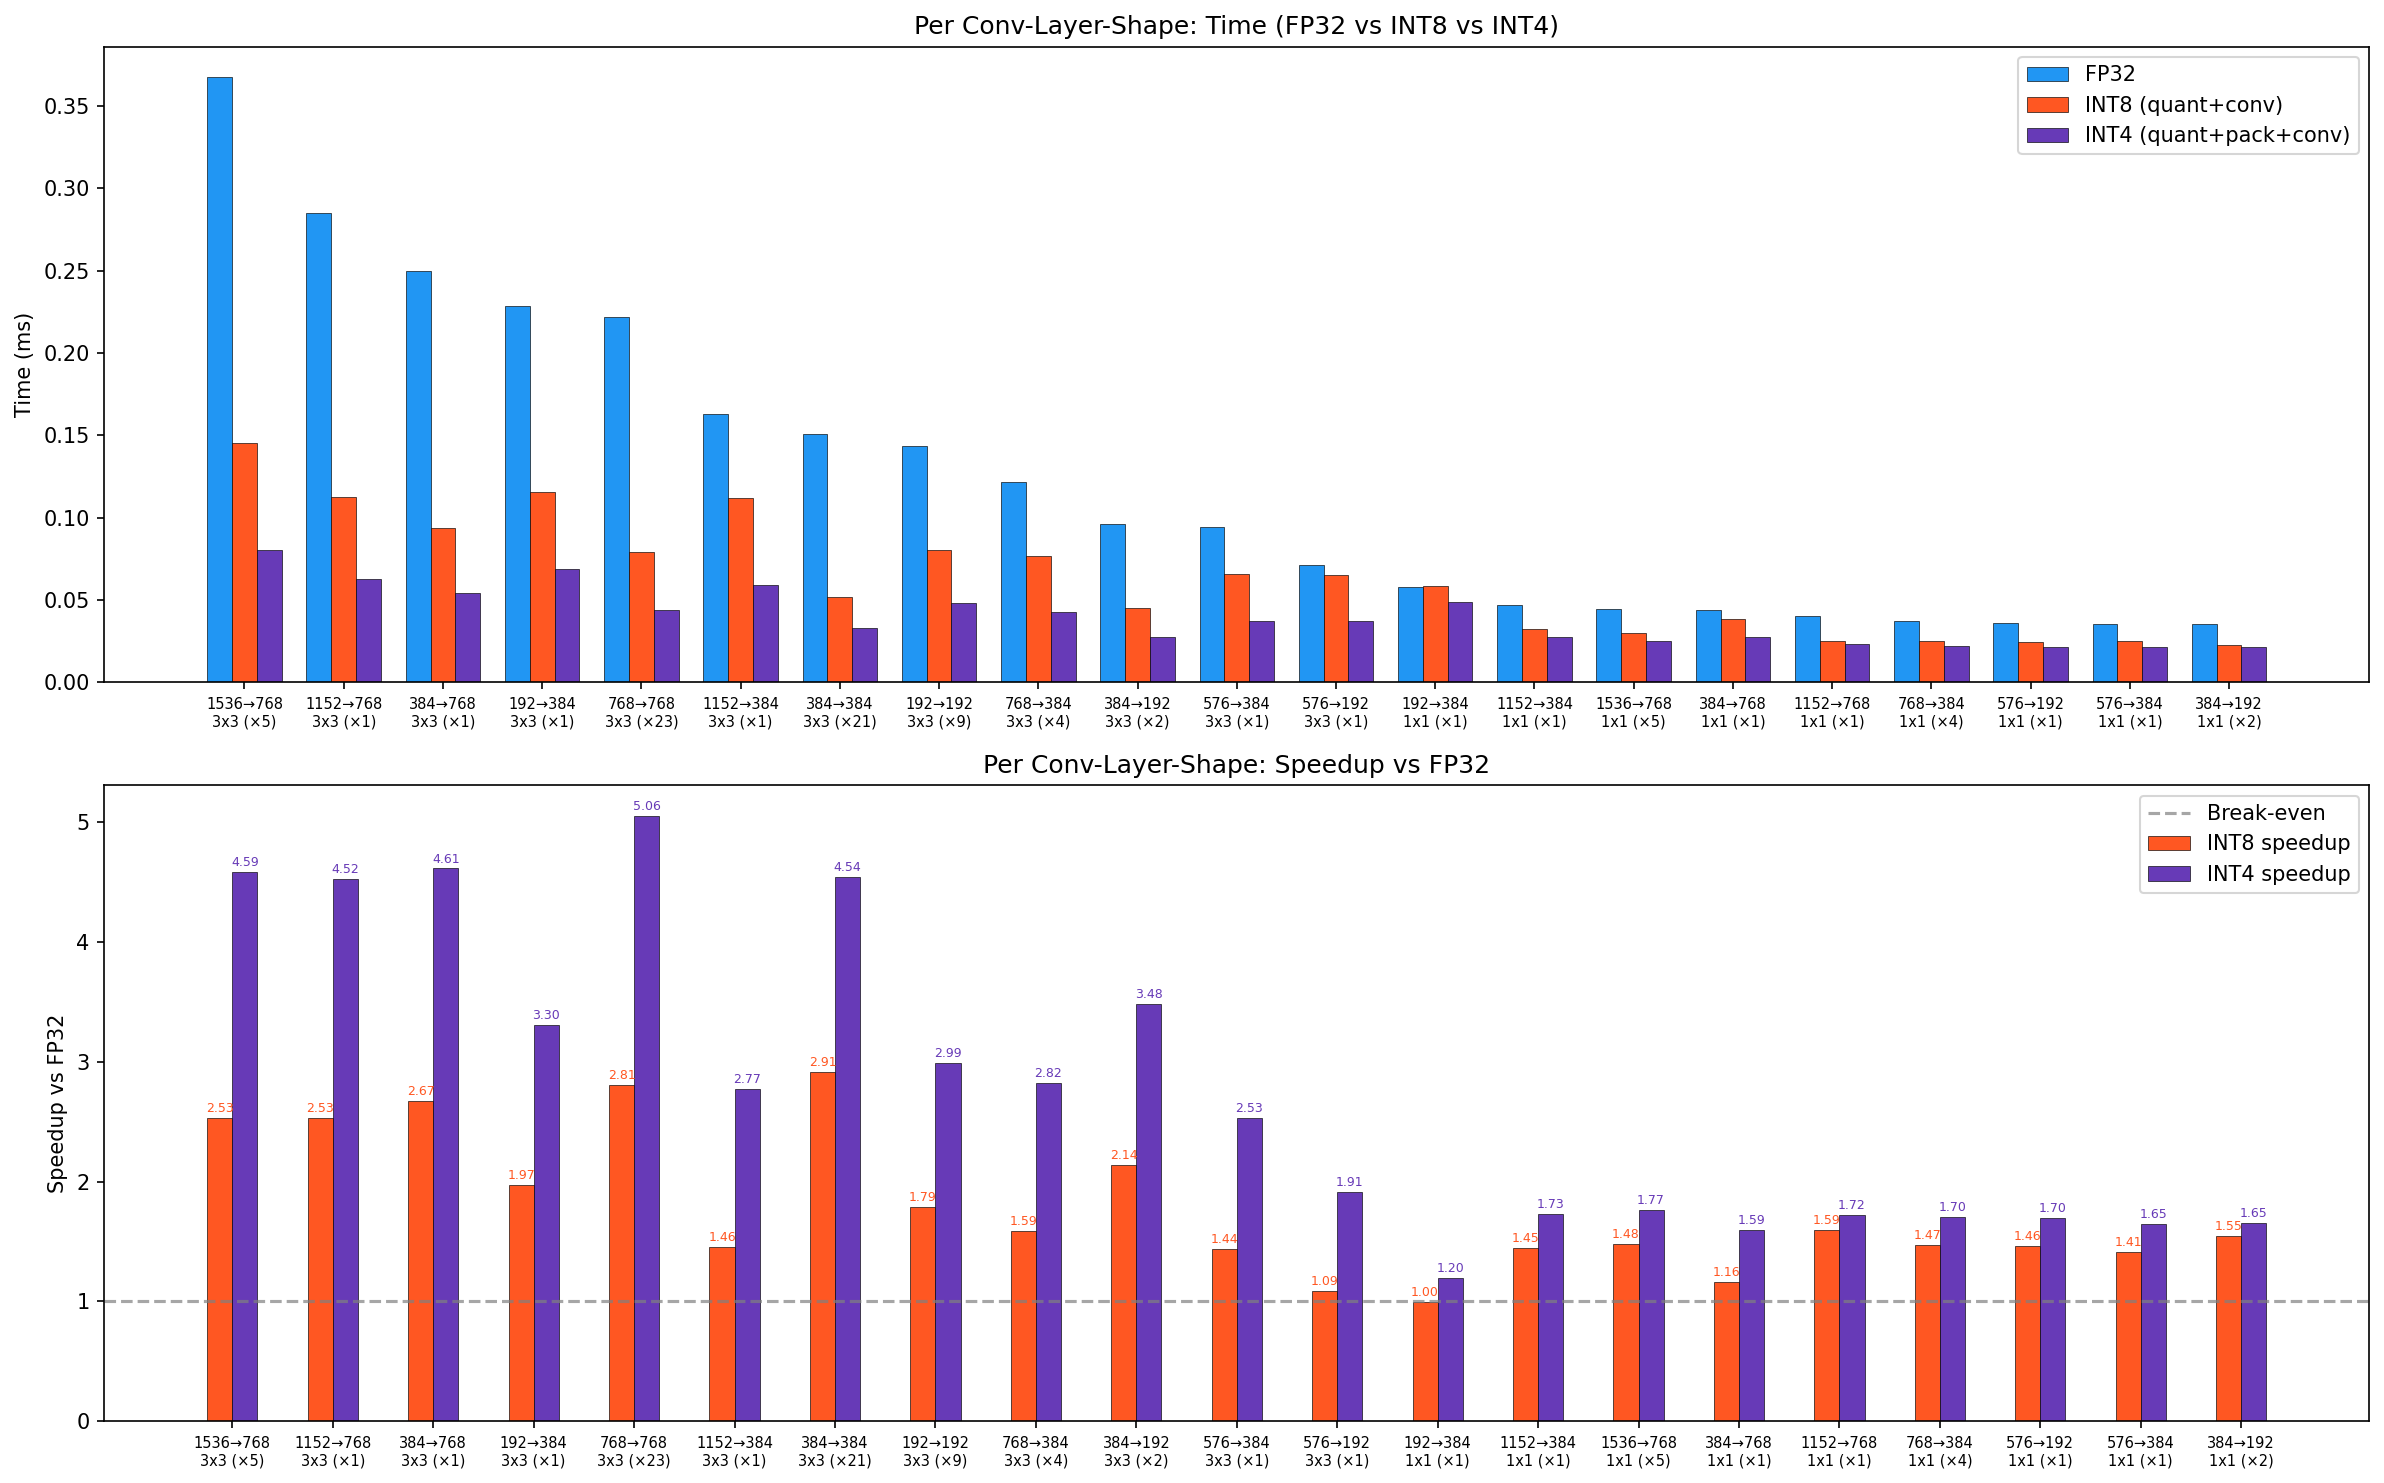
\includegraphics[width=0.80\textwidth]{figures/plot_03_conv_layer_analysis.png}
    \caption{Convolution-layer benchmark across representative UNet shapes.}
    \label{fig:plot_03_conv_layer_analysis}
\end{figure*}
\begin{table}[t]
    \centering
    \caption{Component-wise time cost and speedup. The speedup is compared to FP32.}
    \label{tab:component_breakdown} \resizebox{\linewidth}{!}{
    \begin{tabular}{lr|rr|rr}
        \toprule Component & FP32   & INT8   &       Speedup       & INT4   &      Speedup        \\
        \midrule Conv2d    & 1410.0 & 1355.3 & 1.04$\times$ & 1126.3 & 1.26$\times$ \\
        Attention          & 1378.5 & 750.4  & 1.77$\times$ & 268.8  & 1.84$\times$ \\
        Linear             & 69.4   & 552.4  & 0.13$\times$ & 547.1  & 0.13$\times$ \\
        GroupNorm          & 7.5    & 7.7    & 0.98$\times$ & 60.1   & 1.00$\times$ \\
        SiLU               & 21.1   & 44.4   & 0.48$\times$ & 166.2  & 0.35$\times$ \\
        \bottomrule
    \end{tabular}}
\end{table}

\subsection{Convolutional Layer Benchmark}

To evaluate the CUTLASS-based convolution path and the efficiency of the fused kernels, we benchmark representative UNet conv shapes; results are shown in Figure~\ref{fig:plot_03_conv_layer_analysis}. For most layers, INT8 yields a speedup of approximately $2\times$ to $3\times$, and INT4 achieves up to about $5\times$. The gains are smaller for certain 1$\times$1 layers due to reduced arithmetic work and increased sensitivity to launch and quantization overhead. Through this work, we demonstrate that our kernels achieve significant improvements in computational cost.
